\subsection{Recurrent Convolutional Neural Networks for Discourse Compositionality \cite{Kalchbrenner2013}}

This paper introduces both a sentence model and a discourse model corresponding to the two levels of compositionality: cords combine to form the meaning of sentences, and sentences combine to form the meaning of dialogues. The sentence model adopts convolution as the central operation, and is based on a novel \emph{hierarchical convolutional neural network (HCNN)}. The discourse model extends the sentence model, and is based on a \emph{recurrent neural network (RNN)}.

The basic kernel operation used in HCNN is described as follows. Given a sentence $s$ and its paired matrix $\mathbf{M}^s$, let $\mathbf{m}$ be a feature that is a row in $\mathbf{M}^s$. Let $w_1, ..., w_k$ be a sequence of $k$ weights. The local weighted addition over the first $k$ values is:
$$y = w_1 \mathbf{m}_1 + ... + w_k \mathbf{m}_k.$$
Then a kernel simply defines the value of $k$, and the one-dimensional convolution applies local weighted addition to each subsequence of values of $\mathbf{m}$. The one-dimensional convolution ($\mathbf{k} * \mathbf{m}$) is defined as:
$$(\mathbf{k} * \mathbf{m})_i = \sum_{j=1}^k \mathbf{k}_j \cdot \mathbf{m}_{k+i-j}.$$

To define the hierarchical architecture of the model, the paper next defines a sequence of kernel sizes and associated weights. Let $l$ be the number of words in the sentence $s$. The sequence of kernel sizes is defined as
$$k_1^l = 2, k_{i+1}^l = k_i^l + 1, k_t^l = l - \sum_{j=1}^{t-1}(k_j^l - 1).$$
That is, kernel sizes increase by one until the resulting convolved vector is smaller or equal to the last kernel size (cf. Figure \ref{fig:Kal13-hier}).

\begin{figure}[h]
  \centering
  % Requires \usepackage{graphicx}
  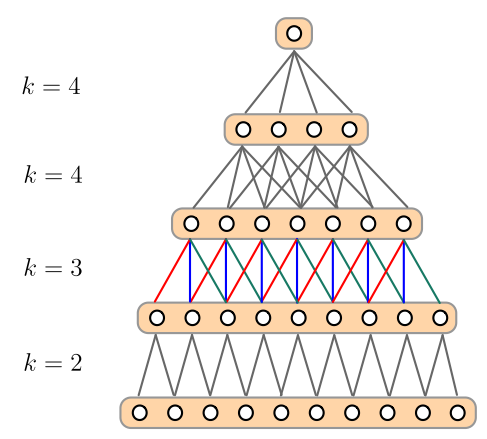
\includegraphics[width=.6\linewidth]{Kal13-hier_HCNN.png}\\
  \caption{A hierarchical convolutional neural network for sentential compositionality.}\label{fig:Kal13-hier}
\end{figure}

The composition operation in HCNN is formally defined as follows. For each feature $f$, let $\mathbf{K}_i^f$ be a sequence of $t$ kernels, where the size of the kernel $|\mathbf{K}_i^f| = k_i^l$. The hierarchy of matrices and corresponding features are defined as:
\begin{align*}
\mathbf{M}_{f,:}^1 &= \mathbf{M}_{f,:}^s,\\
\mathbf{M}_{f.:}^{i+1} &= \sigma(\mathbf{K}_i^f * \mathbf{M}_{f,:}^i + b_f^i).
\end{align*}

The discourse model adapts a RNN architecture in order to capture central properties of discourse. The proposed method aims to capture at least two of the most prominent properties: the sequentiality of the utterances, and the interactions between the speakers.

The RNN architecture takes inputs from a HCNN conditioned on the respective speakers. Let $s_1, ..., s_T$ be a sequence of sentences, each in turn being a sequence of words $s_i = y_1 ... y_l^i$. Let $x_1, ..., x_T$ be a sequence of labels, and $a_1, ..., a_T$ be a sequence of speaker. The RNN computes probability distribution by iterating the following equations:
\begin{align*}
\mathbf{h}_i &= \sigma(\mathbf{I} x_{i-1} + \mathbf{H}^{i-1}\mathbf{h}_{i-1} + \mathbf{Ss}_i + b_h)\\
         p_i &= softmax(\mathbf{O}^i \mathbf{h}_i + b_o)
\end{align*}

\begin{figure}[h]
  \centering
  % Requires \usepackage{graphicx}
  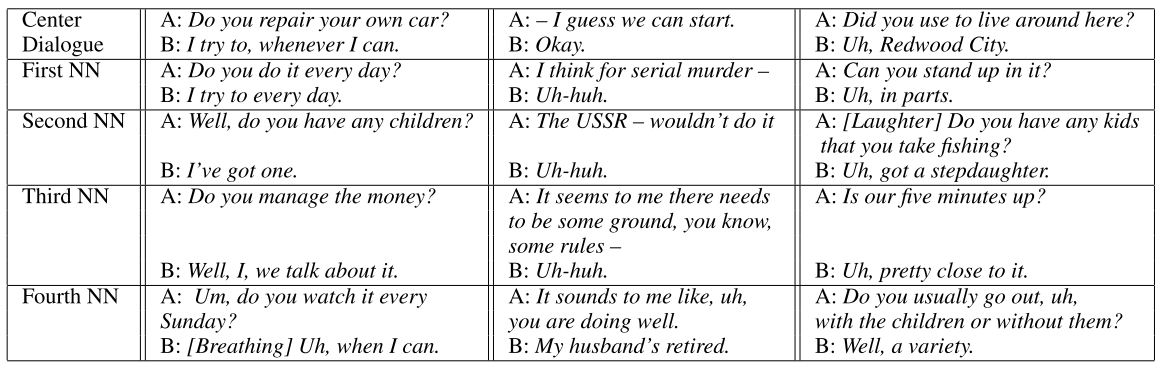
\includegraphics[width=\linewidth]{Kal13-NN.png}\\
  \caption{Short dialogues and nearest neighbours.}\label{fig:Kal13-NN}
\end{figure}

In the experimental study, the paper evaluates the proposed model with the prediction of dialogue acts within the \emph{Switchboard Dialogue Act corpus}. The RCNN model achieves prediction accuracy of 73.9\%, while the best previous result was 71.0\%. Figure \ref{fig:Kal13-NN} shows three randomly chosen dialogues, and the four nearest neighbours of each.
